
\chapter{Internal energy balance} \label{ssn_internal_energy_balance}

The internal energy boundary conditions appropriate to the base of an ice-sheet or glacier are complicated by the fact that both essential and natural types have been specified.  Proposed here is a unification of these conditions in a single natural form, presented as a water content minimization problem whereby an observed maximum value of moisture retention within ice is enforced.  Using this method, previous constraints on the basal energy flux are no longer required, allowing abnormally high intra-ice water contents resulting from internal friction to be drained from the ice using established energy transport equations pertinent to polythermal glaciers.  An algorithm is presented in \S \ref{ssn_dual_optimization} which couples this method with a surface-velocity data-assimilation procedure for basal traction (described in \S \ref{ssn_momentum_optimization_procedure}), resulting in a set fully thermo-mechanically coupled basal traction, velocity, internal energy, and basal water discharge.

\section{Introduction}

Within a polythermal glacier or ice-sheet, both liquid and solid phases are present.  It follows that any mathematical description of polythermal ice must account for the role of liquid water in terms of both rheology and energy.  First, ice is defined as cold if a change in energy leads to a change in temperature alone, and temperate if a change in energy leads to a change in water content alone.  Methods from mixture theory have been incorporated and models proposed which either track the transition surface from cold to temperate \index{Cold/temperate surface} (CTS) explicitly \citep{hutter_1982, greve_1997, greve_2009, blatter_2015}, or solve the internal energy as a single continuous variable \citep{aschwanden_2009, aschwanden_2012}.  Irrespective of the implementation, these models yield a potentially time-varying distribution of internal energy, which via bijection provides temperature and water content.

For cold ice, defined as ice with zero liquid water content, an advection-diffusion equation with a strain-heating source describes heat flow \citep{paterson_1994}. The energy distribution in temperate ice is more complex.  Instead of raising the temperature of ice, strain-heating in these areas generates water.  This water, once produced, is advected along the trajectory of ice flow.  Additionally, the water is thought to either diffuse in the same way as heat \citep{hutter_1982}, as considered here, or move in a similar fashion to groundwater in a Darcy-type pattern whereby pockets of water drain under pressure through micro-connecting veins \citep{fowler_1982}.  The precise mechanism governing the non-advective transport of water remains unclear.

In order to solve equations governing the transport of energy defining these models, appropriate boundary conditions must be prescribed.  Over the surface in contact with atmosphere, estimated water content and temperatures are readily applied as essential-type conditions.  Over the basal surface in contact with bedrock, both geothermal and frictional heat is presented to the ice as a natural-type boundary.  Further complexity arises in imposing this natural boundary condition.

For cold ice, the entirety of geothermal and frictional heat flows into the interior and raises the temperature.  The temperature of ice becomes fixed once it reaches its pressure-melting point, and the energy flux into the ice then becomes proportional to its basal melting rate adjusted by water discharge \citep{greve_1997}.  Additionally, for interior ice with temperature at its pressure-melting point and possessing a non-zero strain-heat source, a \index{Temperate zone} \emph{temperate zone} is created.  While there is no reason a temperate zone could not be formed within the ice interior, the strain-rate is greatest near the bed for ice-sheets and Canadian-type glaciers considered here \citep{aschwanden_2012}, and thus temperate zones typically lie near the basal surface at these localities (Figure \ref{ice_profile_domain}).

As there is no existing constitutive relation explaining the water flux either out of or into the ice in temperate zones, the flux of energy into the ice has been previously specified to be in balance with the flux of water out of the ice, such that a homogeneous natural boundary condition exists \citep{greve_1997, greve_2009, aschwanden_2009, aschwanden_2012, kleiner_2015, blatter_2015}.  In the process of applying this homogeneous energy boundary condition to observed glacial geometries and surface boundary conditions, complications arise when strain-heating creates unreasonably high water content within the ice.  To address this issue, models heretofore have either moved all internally-generated water above a threshold directly into a basal-water storage-layer \citep{greve_1997}, or eliminated some fraction of water at a rate proportional to its magnitude \citep[][section 4.6]{aschwanden_2012}.  In so doing, these models abandon their mathematical formulations in order to ensure that the ice does not deviate from an expected maximum water content. 

The work presented here addresses this shortcoming by expressing the basal boundary condition as a control optimization problem \citep{bryson_1975, nocedal_2000}, whereby an observed maximum basal water content is enforced.  This method is coupled with the basal traction inversion procedure outlined by \citet{macayeal_1993} in order to incorporate satellite- and radar-observed ice surface velocities.  The result of this optimization process is consistent set of of energy, basal water discharge, velocity, pressure, and basal traction fields.  The method is applicable to all diffusive-type energy balance models, requiring only the re-specification of the basal boundary condition and that a method of water transport is available; \ie a non-zero non-advective water flux coefficient is assumed.

%===============================================================================
%===============================================================================

\section{Mathematical foundation}

To begin, the internal energy \index{Internal energy} of ice is defined from the \emph{constitutive equation for internal energy}, as found in \citet{greve_2009},
\begin{align}
  \label{energy}
  \theta(T,W) = \int_{T_0}^T c_i(T') \d{T'} + W L_f,
\end{align}
with absolute temperature $T$, reference temperature $T_0$, and \index{Water content of ice} water content or moisture density $W \in [0,1]$.  Water content $W$ is defined as the ratio of the mass of water contained within a unit-volume of water-ice mixture to the mass of the mixture, such that $W=0$ and $W=1$ corresponds with 100\% ice and 100\% water, respectively.  Energy definition (\ref{energy}) is in turn characterized by the definitions of \index{Heat capacity!Latent} \index{Heat capacity!Sensible} \emph{sensible} heat capacity $c_i$ and \emph{latent} heat capacity $L_f$; the amount of energy required to raise one unit mass of ice one unit of temperature and completely melt one unit mass of ice, respectively.

The \index{Balance equations!Internal energy} \emph{energy balance} takes the form as presented by \citet{greve_1997},
\begin{align}
  \label{energy_balance}
  \rho \totder{\theta}{t} = - \nabla \cdot \rankone{q} + Q,
\end{align}
with mixture density $\rho$, strain-heat $Q$, and energy-flux composed of sensible and latent terms
\begin{align}
  \label{flux}
  \rankone{q} = \rankone{q}_s + \rankone{q}_l,
\end{align}
derived from \emph{Fourier's Law} of conduction \citep{davis_2013}, with thermal conductivity $k$ associated with temperature $T$ and non-advective water flux coefficient $\nu$ associated with water content $W$,
\begin{align}
  \label{individual_flux}
  \rankone{q}_s = - k(\theta) \nabla T \hspace{10mm} 
  \rankone{q}_l = - \nu(\theta) \nabla W.
\end{align}
Note that the energy-dependence of $k$ and $\nu$\footnote{Note here that the latent heat flux coefficient $\nu$ differs from previous formulations such as \citet{greve_1997} and \citet{aschwanden_2012} in that it has multiplicatively absorbed latent heat capacity $L_f$.} make (\ref{energy_balance}) nonlinear.

Bulk water-ice mixture properties apply to thermal conductivity $k$, heat capacity $c$, and density $\rho$,
\begin{align}
  \label{mixture_thermal_conductivity}
  k &= (1-W) k_i + W k_w \\
  \label{mixture_heat_capacity}
  c &= (1-W) c_i + W c_w \\
  \label{mixture_density}
  \rho &= (1-W) \rho_i + W \rho_w,
\end{align}
where the subscripts $i$ and $w$ respectively refer to ice and water.  Thermal conductivity \index{Thermal conductivity} $k_i$ in (\ref{mixture_thermal_conductivity}) has been shown to relate to temperature \citep{yen_1981, ritz_1987, greve_2009},
\begin{align}
  \label{thermal_conductivity}
  k_i = 9.828 \exp\left( -5.7 \times 10^{-3} T \right),
\end{align}
as well as heat capacity $c_i$ in (\ref{mixture_heat_capacity}),
\begin{align}
  \label{heat_capacity}
  c_i = a + b T, \hspace{5mm} a = 146.3, \hspace{5mm} b = 7.253,
\end{align}
while densities $\rho_i$, $\rho_w$ and latent heat properties $k_w$, $c_w$, and $L_f$ are taken as constant.
  
As stated in \citet{hutter_1982, greve_1997, greve_2009, aschwanden_2012}, because the maximum water retention of ice has mostly been observed to be less than 5\% of the total mass, the maximum change in density is less than 0.5\%.  Hence it is reasonable to abandon separate momentum balances for disparate masses of ice and water and instead treat the mixture as a single homogeneous and incompressible fluid.  Thus it is \emph{demanded} that
\begin{align}
  \label{water_demand}
  W \leq W_c \leq 0.05,
\end{align}
where $W_c$ is an observed maximum water content.

Using definition (\ref{heat_capacity}) for heat capacity $c_i$, the integral in energy definition (\ref{energy}) is evaluated using for simplicity $T_0=0$, providing the quadratic equation for energy
\begin{align}
  \label{energy_quad}
  \theta(T,W) &= a T + \frac{b}{2} T^2 + W L_f.
\end{align}

The temperature of ice is also constrained by its melting point, shown to be dependent on pressure $p$ by the \index{Clausius-Clapeyron relationship} \emph{Clausius-Clapeyron} relationship \citep{paterson_1994}
\begin{align}
  \label{temperature_melting}
  T_m = T_w - \gamma p,
\end{align} 
with triple point of water $T_w = 273.15$ and empirically-derived coefficient $\gamma = 9.8 \times 10\sups{-8}$ (represented by the dashed red line in Figure \ref{temperate_zone_revised_image}).  Using this relation, the internal energy of pure ice raised to its pressure-melting point is
\begin{align}
  \label{energy_melting}
  \theta_m = \theta(T_m,0) &= a T_m + \frac{b}{2} T_m^2,
\end{align}
while the internal energy of ice that has been $(W \times 100$)\% melted is
\begin{align}
  \label{temperate_energy}
  \theta(T_m,W) &= \theta_m + W L_f.
\end{align}
Note here that because $0 \leq W \leq 1$, temperatures above the pressure melting point are explicitly forbidden.  This is acceptable, given the very low allowable percentage of water as demanded by (\ref{water_demand}); water internal to the ice will be in close contact with ice and should thus not exceed the melting temperature of ice.

Using (\ref{temperate_energy}), water content $W$ of the mixture is defined as the fraction of internal energy above that of pure ice at the pressure melting point to the specific latent heat of fusion $L_f$,
\begin{align}
  \label{water_content}
  W(\theta) = &\left\{% 
    \begin{array}{ll}
      \frac{\theta - \theta_m}{L_f}, & \theta > \theta_m \\
      0,                             & \theta \leq \theta_m
    \end{array} \right. ,
\end{align}
while temperature $T$ is derived using the quadratic formula with $W=0$ in Equation (\ref{energy_quad}),
\begin{align}
  \label{temperature}
  T(\theta) = &\left\{%
    \begin{array}{ll}
      T_m,                                               & \theta > \theta_m \\
      \frac{-a + \sqrt{a^2 + 2b \theta}}{b}, & \theta \leq \theta_m
    \end{array} \right. .
\end{align}

If a different lower integration bound $T_0$ in (\ref{energy}) were used to calculate (\ref{energy_quad}) and (\ref{energy_melting}) -- say $T_0 = T_m$ at pressure-melting temperature (\ref{temperature_melting}) -- a simple calculation will show that (\ref{energy}) will be negative in areas with temperature below $T_m$, while temperature (\ref{temperature}) and water content (\ref{water_content}) will produce identical values as when taking $T_0 = 0$.  If a more accurate estimate of internal energy is required, one may be attained by using a heat capacity appropriate for the entire range of $T$ from zero to $T_m$, as compiled by \citet{yen_1981}.

Combining energy flux definitions (\ref{flux}) and (\ref{individual_flux}) with definitions of water content (\ref{water_content}) and temperature (\ref{temperature}), the flow of energy may be stated
\begin{align}
  \label{energy_flux_cases}
  \rankone{q} = 
  \begin{cases}
    \rankone{q}_s + \rankone{q}_l = - k \nabla T_m - \nu \nabla W, & \theta > \theta_m \\
    \rankone{q}_s + \rankone{q}_l = - k \nabla T, & \theta \le \theta_m
  \end{cases}.
\end{align}
Because no universally agreed upon constitutive relation exists between latent-energy non-advective flux coefficient $\nu$ and energy $\theta$, the use of the Fickian-type \emph{regularizing} choice of $\nu \approx k / k_0$ for some constant $k_0$ as suggested by \citet{aschwanden_2009} is used here.
The \index{Enthalpy} \index{Enthalpy-gradient method} \emph{enthalpy-gradient} method \citep{pham_1995, aschwanden_2009, aschwanden_2012} simplifies energy-flux term (\ref{energy_flux_cases}) further by using the unified energy flux
\begin{align}
  \label{enthalpy_grad}
  \rankone{q} = - \left( \frac{\kappa}{c} \right) \nabla \theta, \hspace{10mm}
  \kappa =
  \begin{cases}
    \frac{k}{k_0}, & \theta > \theta_m \\
    k,             & \theta \leq \theta_m
  \end{cases}.
\end{align}
Note that for enthalpy $\tilde{\theta}$, the relationship to internal energy $\theta$, pressure $p$, and volume $V$ is \citep{yen_1981}
\begin{align}
  \label{enthalpy}
  \d{\tilde}{\theta} &= \d{\theta} + p \d{V},
\end{align}
and using the same reasoning leading to demand (\ref{water_demand}), for incompressible ice $\d{V} \approx 0$, and therefore enthalpy $\tilde{\theta}$ can be taken synonymously with internal energy $\theta$ in the context of glaciers and ice-sheets.

While the enthalpy-gradient method has been shown to reproduce a nearly identical CTS as models which track the CTS explicitly \citep{kleiner_2015}, great care must be taken when discritizing the system of equations \citep{blatter_2015}.  However, the study here only requires alteration of the basal boundary conditions appropriate to these models, and hence any variability in the CTS caused by either the choice of $k_0$ or the method of discretization of enthalpy-gradient flux (\ref{enthalpy_grad}) may be safely ignored, without losing generality.

The material (convective) derivative and divergence terms in energy-balance (\ref{energy_balance}) are expanded using enthalpy-gradient flux (\ref{enthalpy_grad}),
\begin{align}
  \label{energy_euler_lagrange}
  \rho \left( \parder{\theta}{t} + \rankone{u} \cdot \nabla \theta \right) &= \nabla \left( \frac{\kappa}{c} \right) \cdot \nabla \theta + \frac{\kappa}{c} \nabla \cdot \nabla \theta + Q,
\end{align}
where $\rankone{u} = [u\ v\ w]^\intercal$ is the mixture velocity in Cartesian coordinates with respective horizontal axes $(x,y)$ and vertical $z$ (Figure \ref{ice_profile_domain}).  Note that if a constant heat capacity and thermal conductivity were used, as is commonly done, the first term on the right-hand-side of this equation would be zero and could hence be eliminated.  I prefer to include this temperature relationship, as it accounts for up to 50\% extra variation in diffusive capability (Figure \ref{bulk_thermal_image}).  In the presence of water the ice mixture will be less able to conduct energy due to decreased bulk thermal conductivity (\ref{mixture_thermal_conductivity}), increased bulk heat capacity (\ref{mixture_heat_capacity}), and increased bulk density (\ref{mixture_density}) used with energy-balance (\ref{energy_euler_lagrange}).  This variation in diffusion is measured by dividing both sides of energy balance (\ref{energy_euler_lagrange}) by density $\rho$, resulting in the \index{Diffusivity} \emph{diffusivity}
\begin{align}
  \label{diffusivity}
  \Xi=\kappa/(\rho c),
\end{align}
so named because it is attached to the \emph{diffusive} term $\nabla \cdot \nabla \theta$.

\begin{figure}
  \centering
    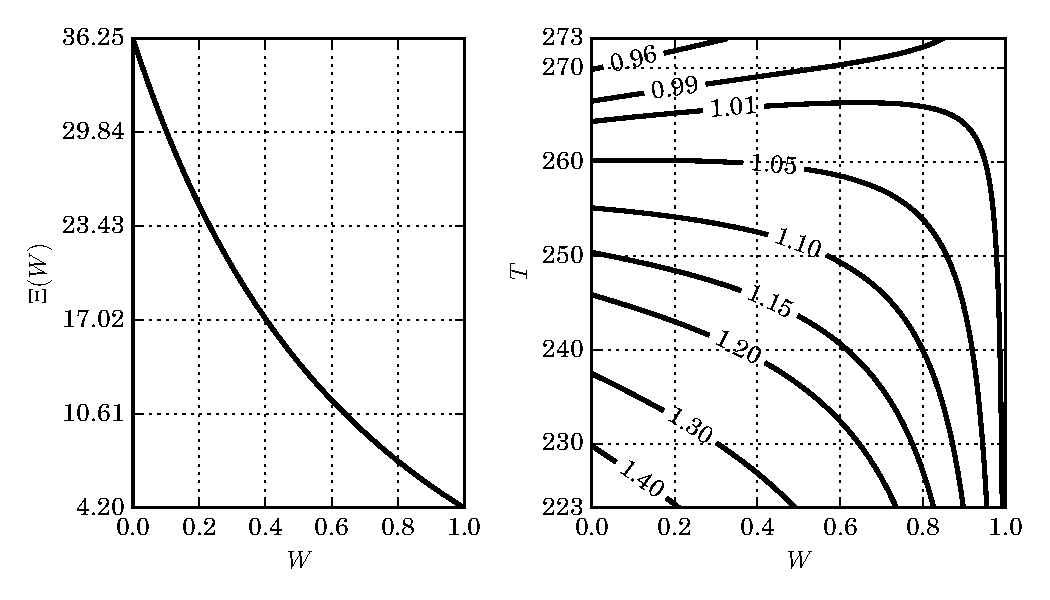
\includegraphics[width=\linewidth]{images/internal_energy/kappa.pdf}
  \caption[Energy diffusivity diagram]{Energy diffusivity $\Xi(W, T=268.15)$ in units of m\sups{2}a\sups{-1} (left) as a function of water content $W$ only, and the ratio of $\Xi(W,T=268.15)$ to $\Xi(W,T)$ (right) utilizing the temperature-dependent heat capacity (\ref{heat_capacity}) and thermal conductivity (\ref{thermal_conductivity}) in diffusivity (\ref{diffusivity}).}
  \label{bulk_thermal_image}
\end{figure}

%===============================================================================
%===============================================================================

\subsection{Momentum interdependence}

Coupling between energy balance (\ref{energy_euler_lagrange}) and momentum balance (\ref{cons_momentum}, \ref{cons_mass}) occurs through pressure-melting relation (\ref{temperature_melting}, \ref{energy_melting}) and friction, both internally with strain-heat (\ref{strain_heat}) and externally with basal fiction heat generated by sliding over rough terrain.

First, shear viscosity (\ref{viscosity}) and internal friction (\ref{strain_heat}) are defined with the Arrhenius-type, energy-dependent flow-rate factor \index{Flow-rate factor} \index{Flow enhancement factor}
\begin{align}
  \label{rate_factor}
  A(\theta) = a_T E \left( 1 + 181.5 W_f \right) \exp\left(-\frac{Q_T}{RT'} \right),
\end{align}
with enhancement factor $E = 1$ unless otherwise specified (see \S \ref{ssn_shelf_inversion}), universal gas constant $R$, empirically-constrained water content $W_f = \min\{W, 0.01\}$ \citep{paterson_1994}, energy-dependent flow-parameter \citep{paterson_1982}
\begin{align}
  \label{flow_parameter}
  a_T &= \begin{cases}
           3.985 \times 10^{-13} \hspace{3mm} \text{s\sups{-1}Pa\sups{-3}} & T' < 263.15 \\
           1.916 \times 10^{3\hphantom{-1}} \hspace{3mm} \text{s\sups{-1}Pa\sups{-3}} & T' \geq 263.15 \\
         \end{cases},
\end{align}
temperature-dependent creep activation energy 
\begin{align}
  \label{activation_energy}
  Q_T & = \begin{cases}
            6.00 \times 10^{4} \hspace{3mm} \text{J mol\sups{-1}} & T' < 263.15 \\
            1.39 \times 10^{5} \hspace{3mm} \text{J mol\sups{-1}} & T' \geq 263.15 \\
          \end{cases},
\end{align}
with pressure-melting adjusted temperature $T' = T + \gamma p$ \citep{greve_2014}.  Note that rate factor (\ref{rate_factor}) will decrease with decreasing temperature, and increase with increasing water content.  This dependence on energy is thus also expressed by shear viscosity (\ref{viscosity}) and internal friction (\ref{strain_heat}).  Therefore, a decrease in energy $\theta$ produces stiffer ice that is more resistance to deformation, while an increase in $\theta$ produces softer ice which is easier to deform (Figure \ref{rate_factor_image}).

The second coupling between energy and momentum is by external friction heat flowing into the ice -- defined analogously to internal friction (\ref{strain_heat}) -- formed from the negative product of \emph{tangential stress} with \emph{tangential velocity} \citep{greve_2009}
\begin{align}
  \label{basal_friction_heat}
  q_{fric} = -\big( \sigma \cdot \normal \big)_{\Vert} \cdot \rankone{u}_{\Vert} = \beta \rankone{u} \cdot \rankone{u} = \beta \Vert \rankone{u} \Vert^2,
\end{align}
where impenetrable bed condition (\ref{impenetrability}) was used.

\begin{figure}
  \centering
    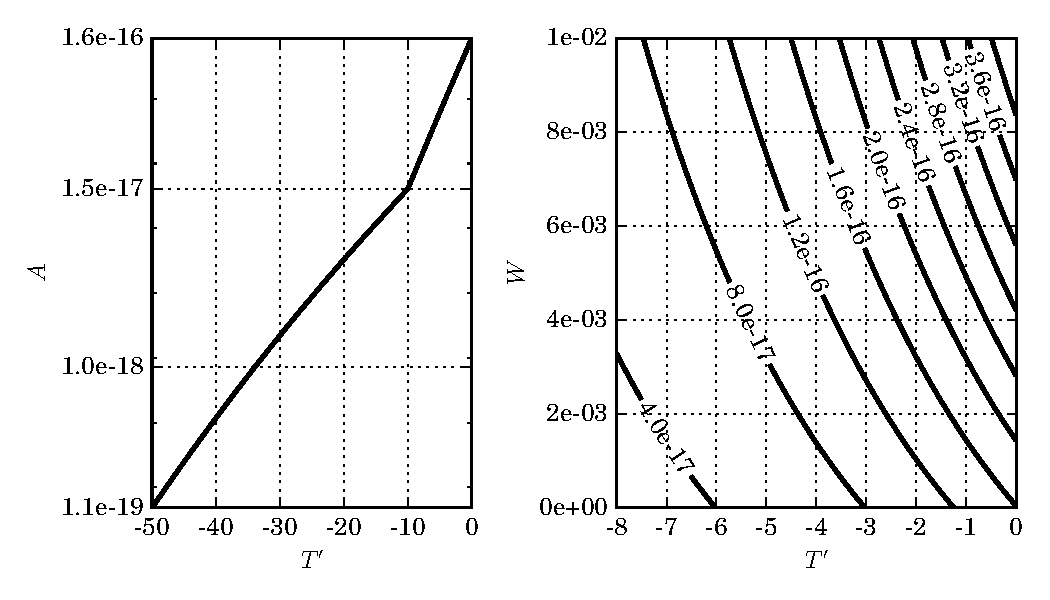
\includegraphics[width=\linewidth]{images/internal_energy/rate_factor_new.pdf}
  \caption[Flow-rate-factor diagram]{Flow rate factor (\ref{rate_factor}) in Pa\sups{-3}a\sups{-1} used in viscosity (\ref{viscosity}) with $W=0$ (left), and a range of water contents (right).  The change in slope in the left figure at $-10^\circ$ C is due the discontinuity of parameters (\ref{flow_parameter}) and (\ref{activation_energy}).}
  \label{rate_factor_image}
\end{figure}


%===============================================================================
%===============================================================================

\section{Energy boundary conditions} \label{ssn_energy_boundary_conditions}

The flow of energy present on the base of the ice, when neglecting sub-glacial water transport, is a combination of geothermal $q_{geo}$ and friction energy from sliding $q_{fric}$ sources
\begin{align}
  \label{basal_energy_source}
  g_N = q_{geo} + q_{fric},
\end{align}
in units of Wm\sups{-2}.  For cold regions this energy flux can only raise the temperature of ice, whereas for ice at its pressure melting point, the energy flux will create water along the basal surface by melting.  Once generated, this water is available for transport via a sub-glacial hydraulic network.  If basal water transport is prohibited, the energy flux will raise the water content along the basal surface, which may then flow under pressure through veins located between ice three-grain boundaries \citep{nye_1973, shreve_1972, raymond_1975, lliboutry_1996}.  The specification of sub-glacial water transport is therefore critical for determining the correct distribution of water -- and thus energy -- both interior and exterior to the ice sheet.  While beyond the scope of study here, basal hydraulic models may be easily incorporated into the solution method presented in the following sections.

The boundary conditions over exterior ice-sheet surface $\Gamma = \Gamma_A \cup \Gamma_W \cup \Gamma_C \cup \Gamma_T$ with atmosphere boundary $\Gamma_A$, boundary in contact with ocean $\Gamma_W$, cold or temperate basal surface without overlying temperate ice $\Gamma_C$, and temperate basal surface with overlying temperate ice $\Gamma_T$ (Figure \ref{ice_profile_domain}) for temperature $T$ are
\begin{align}
  \label{surface_temperature}
  T &= T_S &&\text{ on } \Gamma_A, \\
  \label{sea_temperature}
  T &= T_{sea} &&\text{ on } \Gamma_W, \\
  \label{temperature_flux}
  \big( k \nabla T \big) \cdot \normal &= g_N &&\text{ on } \Gamma_C, \\
  \label{temperate_temperature}
  T &= T_m &&\text{ on } \Gamma_T,
\end{align}
where seawater temperature $T_{sea}$ may possibly be unequal to pressure melting temperature $T_m$.  A similar set of conditions exist for water content $W$,
\begin{align}
  \label{surface_water}
  W &= W_S      &&\text{ on } \Gamma_A, \\
  \label{sea_water_content}
  W &= W_{sea}  &&\text{ on } \Gamma_W, \\
  \label{cold_water}
  W &= 0        &&\text{ on } \Gamma_C, \\
  \label{latent_flux}
  \big( \nu \nabla W \big) \cdot \normal &= \rho L_f M_b - \rho_w L_f F_b  &&\text{ on } \Gamma_T,
\end{align}
with basal melting rate $M_b$, basal water discharge \index{Basal water discharge} from the ice $F_b$, and water content on ocean boundaries $W_{sea}$.  Note that latent energy flux \index{Latent energy flux} (\ref{latent_flux}) has been defined previously by \citet{greve_1997}; make the substitution $\rho_{\text{w}}^+ = \rho_w$, $\mathcal{P}_{\text{b}}^{\text{w}} = \rho M_b$, and $\dot{m}_{\text{b}}^{\text{w}} = \rho_w F_b$ in Equation (2.44) and $\omega^- \approx 0$ in Equation (2.51) of this work (see Appendix A).

The relationship between basal water content and the above stated basal boundary conditions may be put into perspective by considering the \index{Balance equations!Basal energy} \emph{basal energy balance}, defined as a combination of energy flowing into the mixture, sensible energy flux out of the mixture, and energy fluctuations caused by latent heat of fusion transitions \citep[][section 9.3.4]{greve_2009}:
\begin{align}
  \label{basal_energy_balance}
  M_b L_f \rho = q_{geo} + q_{fric} - \big( k \nabla T \big) \cdot \normal &&\text{ on } \Gamma_G,
\end{align}
where $\Gamma_G = \Gamma_C \cup \Gamma_T$ is the entire grounded basal surface.  Note that because $L_f$ and $\rho$ are both positive and non-zero, if $M_b > 0$, mass is able to be accumulated by the basal hydraulic network in the form of melting ice.  Likewise, if $M_b < 0$, the ice is able to accumulate mass on its basal surface in the form of freezing water, if available from the hydraulic network.  Furthermore, note that for $T |_{\Gamma_G} < T_m$, the flux of temperature from the ice (\ref{temperature_flux}) inserted into basal energy balance (\ref{basal_energy_balance}) implies that $M_b = 0$.  Finally, at temperate basal regions, essential temperature condition (\ref{temperate_temperature}) applies and the basal melt rate \index{Basal melting rate} becomes quantifiable from basal energy balance (\ref{basal_energy_balance}),
\begin{align}
  \label{basal_melt_rate}
  M_b = \frac{q_{geo} + q_{fric} - \big( k \nabla T \big) \cdot \normal}{L_f \rho} &&\text{ on } \Gamma_{CT}.
\end{align}
where $\Gamma_{CT} = \left( \Gamma_C \cap \Gamma_T \right) \cup \Gamma_T$ is the entire temperate basal surface.  Therefore, basal melt rate $M_b$ is a means to quantify both the interaction of the ice with sub-glacial water by way of basal melting and accretion by freezing (referred to as \index{Basal freeze-on} \emph{basal freeze-on}), and the flux of water into the base of the ice.  

Similarly, solving for basal water discharge $F_b$ in latent energy flux (\ref{latent_flux}) results in
\begin{align}
  \label{basal_water_discharge}
  F_b &= \frac{\rho L_f M_b - \left( \nu \nabla W \right) \cdot \normal}{L_f \rho_w} &&\text{ on } \Gamma_T.
\end{align}
This is the total rate of water flowing from the ice in units of m s\sups{-1}.  Note that if $F_b = 0$ no amount of water is able to flow from the ice.  In this case, latent energy flux (\ref{latent_flux}) is solely determined by basal melt rate (\ref{basal_melt_rate}) and all basally-generated melt water is available for transport to the interior of the ice as governed by enthalpy gradient flux (\ref{enthalpy_grad}).  Basal water discharge $F_b$ may also be negative, corresponding with water flowing into the ice from the basal hydraulic network, and positive, corresponding with water flowing out; this will respectively increase and decrease latent energy flux (\ref{latent_flux}).  For the purposes of this paper, water is not allowed to flow into the interior of the ice from the basal hydraulic network, corresponding to the requirement $F_b \geq 0$.

Next, temperature boundary conditions (\ref{surface_temperature}, \ref{sea_temperature}) and water boundary conditions (\ref{surface_water}, \ref{sea_water_content}) are combined using energy constitutive relation (\ref{energy}),
\begin{align}
  \label{gamma_a_ebc}
  \theta &= \int_{T_0}^{T_S} c_i(T') \d{T'} + W_S L_f &&\text{ on } \Gamma_A \\
  \label{gamma_w_ebc}
  \theta &= \int_{T_0}^{T_{sea}} c_i(T') \d{T'} + W_{sea} L_f &&\text{ on } \Gamma_W,
\end{align}
which may be evaluated using Equation (\ref{energy_quad}) if $T_0 = 0$.

Basal regions containing overhead temperature at the temperature melting point $T_m$ are defined by the coefficient
\begin{align}
  \label{weak_temperate_marker}
  \alpha_w = \begin{cases}
             0, & \nabla T \cdot \normal \neq \nabla T_m \cdot \normal \hspace{2.5mm} \text{ on } \Gamma_G \\
             1, & \nabla T \cdot \normal = \nabla T_m \cdot \normal \hspace{2.5mm} \text{ on } \Gamma_G 
           \end{cases},
\end{align}
or, using the continuity of internal water content $W$, by the coefficient
\begin{align}
  \label{temperate_marker}
  \alpha = \begin{cases}
             0, & W = 0 \hspace{2.5mm} \text{ on } \Gamma_G \\
             1, & W > 0 \hspace{2.5mm} \text{ on } \Gamma_G 
           \end{cases}.
\end{align}
Coefficient (\ref{temperate_marker}) is stronger than (\ref{weak_temperate_marker}), as it does not require calculation of derivatives and is thus not affected by low-resolution approximation errors arising from the discretization.

Coefficient (\ref{temperate_marker}) used in conjunction with enthalpy-gradient flux (\ref{enthalpy_grad}) and basal melt rate (\ref{basal_melt_rate}) combines sensible energy flux (\ref{temperature_flux}) and latent energy flux (\ref{latent_flux}) over the entire grounded surface $\Gamma_G$:
\begin{align}
  \label{temperate_flux}
  \left( \frac{\kappa}{c} \nabla \theta \right) \cdot \normal &= \begin{cases}
             g_N, & \alpha = 0  \\
             g_N - (k \nabla T_m) \cdot \normal - \rho_w L_f F_b, & \alpha = 1
           \end{cases},
\end{align}
producing finally the basal energy flux
\begin{align}
  \label{energy_flux}
  \left( \frac{\kappa}{c} \nabla \theta \right) \cdot \normal
  &= g_N - \alpha g_W &&\text{ on } \Gamma_G,
\end{align}
where $g_W = (k \nabla T_m) \cdot \normal + \rho_w L_f F_b$.  By stating basal energy flux boundary (\ref{energy_flux}) in this manner, a continuous range of basal energy flux values across the entire grounded basal surface is allowed.

In areas with overlying temperate ice, it has been previously assumed \citep{aschwanden_2012, kleiner_2015} that the flux of water -- and therefore energy -- out of the ice is in balance with the water gradient caused by basal melt, corresponding with the condition $F_b=M_b \rho / \rho_w$ in energy-flux (\ref{energy_flux}) and
\begin{align}
  \label{zero_basal_water_discharge}
  \left( \frac{\kappa}{c} \nabla \theta \right) \cdot \normal &= g_N - \alpha g_N &&\text{ on } \Gamma_G.
\end{align}
By the strict use of this boundary condition, strain-heating may increase the water content of interior ice to abnormally high levels \citep{aschwanden_2012}.  In contrast, by using generalized basal energy flux (\ref{energy_flux}) while allowing the possibility for $F_b > M_b \rho / \rho_w$, the energy flux across the basal surface is able to adapt to large quantities of internally-generated water produced by internal friction (\ref{strain_heat}).

Therefore, provided that the non-advective water-flux coefficient $\nu$ in water flux (\ref{latent_flux}) is greater than zero -- corresponding to an enthalpy-gradient coefficient (\ref{enthalpy_grad}) with $k_0 < \infty$ in temperate regions -- a procedure for choosing an appropriate value of $F_b$ in (\ref{energy_flux}) defines a mechanism for enforcing maximum water retention demand (\ref{water_demand}).


%===============================================================================
%===============================================================================

\section{Exploring basal-melting-rate}

\index{Basal melting rate}
As discussed in \S \ref{ssn_energy_boundary_conditions}, basal melting rate (\ref{basal_melt_rate}) is only valid in regions where $\theta \ge \theta_m$ and is positive only when
\begin{align}
  q_{geo} + q_{fric} > \big( k_i \nabla T_m \big) \cdot \normal.
\end{align}
Digging deeper into the pressure-melting gradient,
\begin{align}
  \big( k_i \nabla T_m \big) \cdot \normal &= \big( k_i \gamma \nabla p \big) \cdot \normal \notag \\
  &= k_i \gamma \nabla \big( \delta p \big) \cdot \normal + k_i \gamma \big( \nabla (\rho g (S - z)) \big) \cdot \normal \notag \\
  &= k_i \gamma \nabla \big( \delta p \big) \cdot \normal + k_i \gamma \rho g \left( \parder{S}{x} n_x + \parder{S}{y} n_y  + n_z \right) \notag,
\end{align}
where Clausius-Clapeyron relationship (\ref{temperature_melting}) has been applied and basal pressure $p$ was separated into cryostatic $\rho g H$ with $z$-varying thickness $H = S - z$ for surface height $S$, and dynamic $\delta p$ terms \index{Pressure!cryodynamic} \index{Pressure!cryostatic} .  Next, applying the low basal-slope requirement of first-order momentum \citet{blatter_1995, pattyn_2003}, $\normal \approx [0\ 0\ \text{-}1]^\intercal$ and
\begin{align}
  \big( k_i \nabla T_m \big) \cdot \normal
  &\approx - k_i \gamma \frac{\partial \delta p}{\partial z} - k_i \gamma \rho g = - k_i \gamma \left( \frac{\partial \delta p}{\partial z} + \rho g \right).
\end{align}
Therefore, because $q_{geo}$ and $q_{fric}$ (\ref{basal_friction_heat}) are both positive-definite functions, refreeze only occurs in regions where the dynamic pressure gradient is able to overcome the geothermal and frictional energy flux adjusted by a small scalar value,
\begin{align}
  \label{refreeze}
  q_{geo} + q_{fric} > k_i \gamma \left( \frac{\partial \delta p}{\partial z} + \rho g \right) \implies \text{ refreezing.}
\end{align}
Note also that in the case of cryostatic assumptions, $\delta p$ is zero and refreeze condition (\ref{refreeze}) simplifies to $q_{geo} + q_{fric} > k_i \gamma \rho g$.  Hence with an average geothermal flux of $\mathcal{O}(10\sups{-2})$ W m\sups{-2}, $q_{fric} \gg q_{geo}$, and $k_i \gamma \rho g = \mathcal{O}(10\sups{-3})$ W m\sups{-2}, refreeze is unlikely to occur under these assumptions.  Therefore, the full-Stokes momentum balance must be applied in order to properly identify refreezing or melt.


%===============================================================================
%===============================================================================

\section{Weak energy approximation}

The variational and weak form of the steady-state ($\partial_t \theta = 0$) version of  energy balance (\ref{energy_euler_lagrange}) and associated boundary conditions (\ref{gamma_a_ebc}, \ref{gamma_w_ebc}, \ref{energy_flux}) is constructed by taking the inner product of the residual 
\begin{align}
  \label{energy_forward_model}
  \mathscr{R}(\theta, F_b) &= \rho \rankone{u} \cdot \nabla \theta - \nabla \left( \frac{\kappa}{c} \right) \cdot \nabla \theta - \frac{\kappa}{c} \nabla \cdot \nabla \theta - Q.
\end{align}
with the test function $\psi \in \testspace$ (see test space (\ref{test_space})), integrating over the entire ice-sheet volume $\Omega$,
\begin{align}
  - \int_{\Omega} Q \psi \d{\Omega}
  + \int_{\Omega} \rho \rankone{u} \cdot \nabla \theta \psi \d{\Omega} 
  - \int_{\Omega} \nabla \left( \frac{\kappa}{c} \right) \cdot \nabla \theta \psi \d{\Omega} & \notag \\
  + \int_{\Omega} \left( \frac{\kappa}{c} \right) \nabla \theta \cdot \nabla \psi \d{\Omega} 
  \label{ie_intermediate_var_form}
  - \int_{\Gamma} \left( \frac{\kappa}{c} \nabla \theta \right) \cdot \normal \psi \d{\Gamma} &= 0,
\end{align}
where the diffusive term has been integrated by parts.  Because outward flux terms over essential boundaries vanish (see test space (\ref{test_space})), the boundary integral over $\Gamma$ is reduced to an integral over $\Gamma_G$ using energy flux (\ref{energy_flux}),
\begin{align}
  \label{energy_basal_boundary_form}
  \int_{\Gamma} \left( \frac{\kappa}{c} \nabla \theta \right) \cdot \normal \psi \d{\Gamma} &= \int_{\Gamma_G} \left( g_N - \alpha g_W \right)\ \psi \d{\Gamma_G}.
\end{align}

%===============================================================================

\subsection{Numerical stabilization}

Numerical instabilities will manifest in areas where the transport of energy is dominated by advection (see \S \ref{ssn_stabilized_methods}).  Hence stabilization is required to reduce non-physical oscillations resulting from solving Galerkin-form (\ref{ie_intermediate_var_form}).

To begin, the linear differential operator associated with problem (\ref{energy_euler_lagrange}) is
\begin{align}
  \label{internal_energy_linear_operator}
  \Lu \theta &= \rho \rankone{u} \cdot \nabla \theta - \nabla \left( \frac{\kappa}{c} \right) \cdot \nabla \theta - \frac{\kappa}{c} \nabla \cdot \nabla \theta.
\end{align}
On close inspection, the advective part of this operator is
\begin{align}
  \label{internal_energy_advective_operator}
  \Lu_{\text{adv}} \theta &= \tilde{\rankone{u}} \cdot \nabla \theta,
\end{align}
with quasi-velocity
\begin{align}
  \label{internal_energy_quasi_velocity}
  \tilde{\rankone{u}} &= \rho \rankone{u} - \nabla \left( \frac{\kappa}{c} \right).
\end{align}
The conductive gradient term $\nabla \left( \nicefrac{\kappa}{c} \right)$ of the energy-flux therefore contributes in an advective sense to the transport of energy; energy transport increases as the magnitude of the conductive gradient increases.  For example, if the ice is taken -- without loss of generality -- as stationary, $\rankone{u} = \rankone{0}$ and energy transport occurs by diffusion and quasi-advection in the down-gradient direction of the conduction term $\nicefrac{\kappa}{c}$.

Next, the stabilized form of internal-energy balance (\ref{ie_intermediate_var_form}) with linear operator (\ref{internal_energy_linear_operator}) using general stabilized form (\ref{generalized_form}) with test function $\psi$ and intrinsic-time parameter $\tau_{\text{IE}}$ is 
\begin{align}
  \label{internal_energy_generalized_form}
  (\psi, \Lu \theta) + (\mathbb{L} \psi, \tau_{\text{IE}}(\Lu\theta - Q)) &= (\psi, Q),
\end{align}
where operator $\mathbb{L}$ is a differential operator chosen from 
\begin{align}
  \label{ie_gls_operator}
  \mathbb{L} &= + \Lu && \text{Galerkin/least-squares (GLS)} \\
  \label{ie_supg_operator}
  \mathbb{L} &= + \Lu_{\text{adv}} && \text{SUPG} \\
  \label{ie_ssm_operator}
  \mathbb{L} &= - \Lu^* && \text{subgrid-scale model (SSM)}
\end{align}
with adjoint of operator $\Lu$ denoted $\Lu^*$.

Making the appropriate substitutions in SUPG parameter (\ref{tau_supg}) results in the intrinsic-time parameter \index{Intrinsic-time parameter!Internal energy}
\begin{align}
  \label{tau_ie}
  \tau_{\text{IE}} &= \frac{h \xi(P_{\'e})}{2 \Vert \tilde{\rankone{u}} \Vert}, \hspace{10mm} P_{\'e} = \frac{h \Vert \tilde{\rankone{u}} \Vert}{2 \rho \Xi},
\end{align}
where $h$ is the cell diameter, $P_{\'e}$ is the ratio of advective to diffusive flux coefficients, referred to as the \index{Peclet@P\`eclet number!Internal energy} \emph{element P\'eclet} number, and $\xi(P_{\'e})$ is a function that is dependent on the element-shape-functions utilized.  For example, if the shape functions $\psi$ are taken as the linear Lagrange elements described in \S \ref{ssn_intro_galerkin_equations}, the accuracy-optimal function choice for $\xi$ is given by \citep{brooks_1982}
\begin{align}
  \label{intrinsic_time_ftn}
  \xi\left( P_{\'e} \right) &= \coth \left( P_{\'e} \right) - \frac{1}{P_{\'e}}.
\end{align}
It was later determined by \citet{codina_1992} that when quadratic shape functions are used, the accuracy-optimal function for $\xi$ changes to
\begin{align}
  \xi_1(P_{\'e}) &= \frac{1}{2} \left( \coth\left( \frac{P_{\'e}}{2} \right) - \frac{2}{P_{\'e}} \right) \notag \\
  \label{intrinsic_time_ftn_quad}
  \xi\left( P_{\'e} \right) &= \frac{\big(3 + 3 P_{\'e} \xi_1\big) \tanh(P_{\'e}) - \big(3 P_{\'e} + P_{\'e}^2 \xi_1 \big)}{ \big(2 - 3 \xi_1 \tanh(P_{\'e}) \big) P_{\'e}^2}.
\end{align}
Note that for any substantial ice flow, $P_{\'e}$ will be very large and thus $\xi \approx 1$ (Figure \ref{peclet_image}).  Additionally, note that if linear-Lagrange elements are used, the application of SUPG stabilization (\ref{ie_supg_operator}) and GLS stabilization (\ref{ie_gls_operator}) in form (\ref{internal_energy_generalized_form}) are identical.

Therefore, using boundary integral (\ref{energy_basal_boundary_form}) with variational form (\ref{ie_intermediate_var_form}) in stabilized form (\ref{internal_energy_generalized_form}), the problem consists of finding $\theta \in \mathcal{H}^1(\Omega)$ such that
\begin{align}
  \label{var_form}
  - \int_{\Omega} Q \psi \d{\Omega}
  + \int_{\Omega} \rho \rankone{u} \cdot \nabla \theta \psi \d{\Omega} 
  - \int_{\Omega} \nabla \left( \frac{\kappa}{c} \right) \cdot \nabla \theta \psi \d{\Omega} & \notag \\
  + \int_{\Omega} \left( \frac{\kappa}{c} \right) \nabla \theta \cdot \nabla \psi \d{\Omega} 
  - \int_{\Gamma_G} \left( g_N - \alpha g_W \right)\ \psi \d{\Gamma_G} & \notag \\
  + \int_{\Omega} \tau_{\text{IE}} \big( \mathbb{L} \psi \big) \big( \Lu\theta - Q \big) \d{\Omega} - \int_{\Omega} Q\ \psi \d{\Omega}  &= 0,
\end{align}
for all $\psi \in \mathcal{H}^1(\Omega)$ subject to the remaining essential boundary conditions (\ref{gamma_a_ebc}) and (\ref{gamma_w_ebc}). 

\begin{figure}
  \centering
    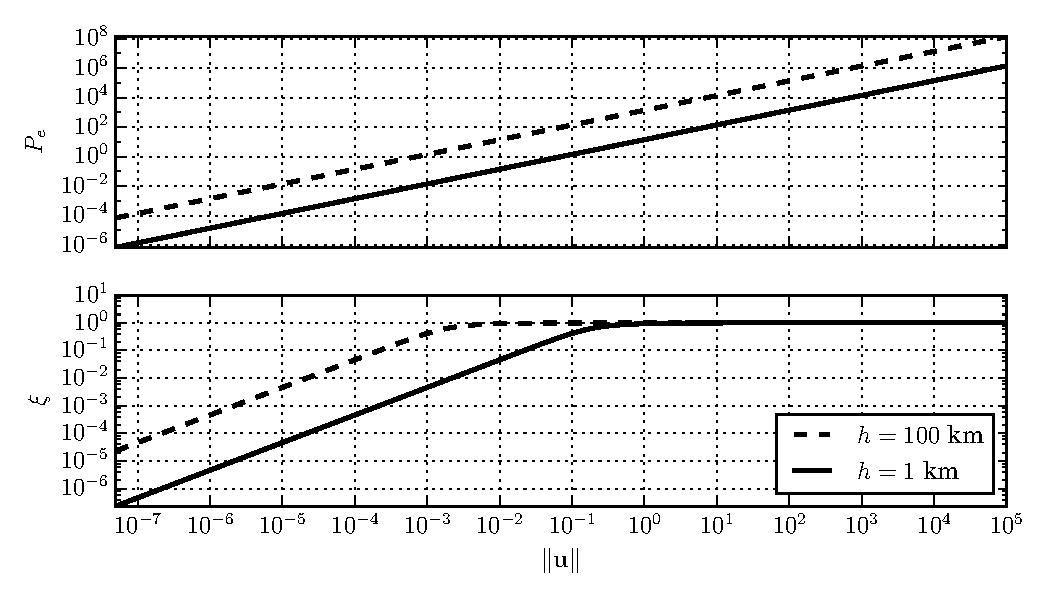
\includegraphics[width=\linewidth]{images/internal_energy/alpha_new.pdf}
  \caption[P\'eclet number and intrinsic-time parameter diagram]{The element P\'eclet number $P_{\'e}$ (top) with $h = 1$ km (solid) and $h=100$ km (dashed) over a range of velocity values with magnitude $\Vert \rankone{u} \Vert$ in m a\sups{-1} appropriate to ice-sheets. The corresponding intrinsic time $\xi$ multiplicative term to the SUPG formulation for linear-Lagrange elements (\ref{intrinsic_time_ftn}) (bottom) becomes very close to unity after the ice speed gets above $\Vert \rankone{u} \Vert \approx 2$ cm a$^{-1}$ with $h=1$ km.}
  \label{peclet_image}
\end{figure}

%===============================================================================

\subsection{Energy balance discretization}

For a mesh with $N_n$ vertices and $N_{\Gamma}$ essential exterior vertices corresponding with Dirichlet boundaries (\ref{gamma_a_ebc}, \ref{gamma_w_ebc}), the approximation 
\begin{align}
  \label{galerkin_approximation}
  \theta \approx \theta_h = \sum_{j=1}^{N_n} \coefvec{\theta}_j \psi_j + \sum_{j=N_n+1}^{N_n+N_{\Gamma}} \coefvec{\theta}_j \psi_j
\end{align}
defines an expansion of $\theta$ with unknown coefficients $\coefvec{\theta}_j$ associated with the trial functions $\psi_j$ (see trial space (\ref{trial_space})). Inserting approximation (\ref{galerkin_approximation}) into (\ref{var_form}) results in the matrix-vector set of equations
\begin{align}
  \label{component_var_form}
  \rankone{r} = \ranktwo{\mathcal{C}}\coefvec{\theta} - \ranktwo{\mathcal{K}}\coefvec{\theta} + \ranktwo{\mathcal{D}}\coefvec{\theta} + \ranktwo{\mathcal{S}} \coefvec{\theta} + \rankone{f}^{\text{ext}} - \rankone{f}^{\text{int}} - \rankone{f}^{\text{stz}},
\end{align}
where for each test function $\psi_i$ with $i,j = 1, 2, \ldots, N_n$,
\begin{align}
  \label{advective_form}
  \mathcal{C}_{ij} &= \int_{\Omega} \rho \rankone{u} \cdot \nabla \psi_j\ \psi_i \d{\Omega} &&\leftarrow \text{advection} \\
  \label{conductive_gradient_form}
  \mathcal{K}_{ij} &= \int_{\Omega} \nabla \left( \frac{\kappa}{c} \right) \cdot \nabla \psi_j\ \psi_i \d{\Omega} &&\leftarrow \text{cond.~grad.} \\
  \label{diffusion_form}
  \mathcal{D}_{ij} &= \int_{\Omega} \left( \frac{\kappa}{c} \right) \nabla \psi_j \cdot \nabla \psi_i \d{\Omega} &&\leftarrow \text{diffusion} \\
  \label{stabilization_form_a}
  \mathcal{S}_{ij} &= \int_{\Omega} \tau_{\text{IE}} \big( \mathbb{L} \psi_i \big) \big( \Lu \psi_j \big) \d{\Omega} &&\leftarrow \text{stab'z'tion} \\
  \label{basal_energy_gradient_form}
  f_i^{\text{ext}} &= \int_{\Gamma_G} \left( g_N - \alpha g_W \right)\ \psi_i \d{\Gamma_G} &&\leftarrow \text{energy flux} \\
  \label{internal_friction_form}
  f_i^{\text{int}} &= \int_{\Omega} Q\ \psi_i \d{\Omega} &&\leftarrow \text{strain heat} \\
  \label{stabilization_form_l}
  f_i^{\text{stz}} &= \int_{\Omega} \tau_{\text{IE}} \big( \mathbb{L} \psi_i \big)\ Q \d{\Omega} &&\leftarrow \text{stab'z'tion},
\end{align}
and $\rankone{r}$ is the residual error vector, defining a \emph{weak solution} $\rankone{\theta}_h$ to variational form (\ref{var_form}) when $\Vert \rankone{r} \Vert = 0$.  When using approximation (\ref{galerkin_approximation}), the sum involving the $N_{\Gamma}$ exterior vertices will produce a set of matrices with identical properties as (\ref{advective_form} -- \ref{diffusion_form}), but where the unknown coefficients $\rankone{\theta}_j$, $j = N_n+1,N_n+2,\ldots,N_n+N_{\Gamma}$ are  known from the surface essential boundaries (\ref{gamma_a_ebc} -- \ref{gamma_w_ebc}).  Thus, the last sum in approximation (\ref{galerkin_approximation}) interpolates the boundary data onto the finite-element basis \citep{elman_2005}.

If an identical discrete basis is used for both $\psi_i$ and $\psi_j$, $\theta_h$ defined by (\ref{galerkin_approximation}) corresponds with \emph{Bubnov-Galerkin} approximation.  In such a case, it is easily seen that $\ranktwo{\mathcal{D}}$ is symmetric, and as it turns out, positive-definite \citep{elman_2005}.  The same cannot be said of $\ranktwo{\mathcal{C}}$ and $\ranktwo{\mathcal{K}}$.  However, symmetry is added back to linear system (\ref{component_var_form}) by the term $\ranktwo{\mathcal{S}}$.  For example, if linear Lagrange elements are used as a basis for $\psi$ and streamline-upwind/Petrov-Galerkin stabilization operator (\ref{ie_supg_operator}) is used,
{\small
\begin{align}
  \label{stabilization_form_a_expanded}
  \ranktwo{\mathcal{S}}_{ij} &= \int_{\Omega} \tau_{\text{IE}} \big( \Lu_{\text{adv}} \psi_i \big) \big( \Lu \psi_j \big) \d{\Omega} \notag \\
  &= \int_{\Omega} \tau_{\text{IE}} \left( \left( \rho \rankone{u} + \nabla \left( \frac{\kappa}{c} \right) \right) \cdot \nabla \psi_i \right) \left( \left( \rho \rankone{u} + \nabla \left( \frac{\kappa}{c} \right) \right) \cdot \nabla \psi_j \right) \d{\Omega} \notag \\
  &= \int_{\Omega} \tau_{\text{IE}} \left( \tilde{\rankone{u}} \cdot \nabla \psi_i \right) \left( \tilde{\rankone{u}} \cdot \nabla \psi_j \right) \d{\Omega},
\end{align}}
where quasi-velocity (\ref{internal_energy_quasi_velocity}) has been applied and the fact that second-derivatives of linear element shape-functions are zero.  Matrix (\ref{stabilization_form_a_expanded}) is symmetric-positive-definite, and thus the addition of this term in (\ref{component_var_form}) has the effect of increasing the stability or \emph{coercivity} of the linear system.

An algorithm well suited for the solution of problems possessing non-symmetric matrices such as these is the \emph{generalized minimum residual method} (GMRES).  This procedure is one of many \emph{Krylov subspace methods}, which iteratively reduces the energy norm of the error.  However, because the non-advective flux coefficient $\kappa$ is discontinuous, depending on the unknown $\coefvec{\theta}$, and also because thermal properties (\ref{thermal_conductivity}) and (\ref{heat_capacity}) are non-linear with respect to $\coefvec{\theta}$, system (\ref{component_var_form}) is non-linear.  Thus, a linearization of this system is required.  One such linearization is \emph{Newton's method}, which iteratively reduces residual (\ref{component_var_form}) by solving for the direction of decent with respect to the solution space of $\theta$ (investigate \S \ref{ssn_newton_raphson}).

The source code of \CSLVR uses an implementation similar to Code Listing \ref{cslvr_enthalpy}.

\begin{python}[label=cslvr_enthalpy, caption={\CSLVR source code contained in the \texttt{Enthalpy} class.}]
# define test and trial functions : 
psi     = TestFunction(model.Q)
dtheta  = TrialFunction(model.Q)
theta   = Function(model.Q, name='energy.theta')
  
# momentum-dependent properties :
U       = momentum.velocity()
epsdot  = momentum.effective_strain_rate(U) + model.eps_reg
eta     = momentum.viscosity(U)
    
# internal friction (strain heat) :
Q_s     = 4 * eta * epsdot

# coefficient for non-advective water flux (enthalpy-gradient) :
k_c     = conditional( gt(W, 0.0), model.k_0, 1 )

# thermal conductivity and heat capacity (Greve and Blatter 2009) :
ki      = 9.828 * exp(-0.0057*T)
ci      = 146.3 + 7.253*T

# bulk properties :
k       =  (1 - W)*ki   + W*kw     # bulk thermal conductivity
c       =  (1 - W)*ci   + W*cw     # bulk heat capacity
rho     =  (1 - W)*rhoi + W*rhow   # bulk density
kappa   =  spy * k_c * k           # discontinuous with water, J/(a*m*K)
Xi      =  kappa / (rho*c)         # bulk enthalpy-gradient diffusivity

# basal heat-flux natural boundary condition :
q_fric  = beta * inner(U,U)
g_w     = model.gradTm_B + rhow*L*Fb
g_n     = q_geo + q_fric
g_b     = g_n - alpha*g_w

# the Peclet number : 
Ut     = rho*U - grad(kappa/c)
Unorm  = sqrt(dot(Ut, Ut) + DOLFIN_EPS)
PE     = Unorm*h/(2*kappa/c)

# for linear elements :
if model.order == 1:
  xi     = 1/tanh(PE) - 1/PE

# for quadratic elements :
if model.order == 2:
  xi_1  = 0.5*(1/tanh(PE) - 2/PE)
  xi    =     ((3 + 3*PE*xi_1)*tanh(PE) - (3*PE + PE**2*xi_1)) \
           /  ((2 - 3*xi_1*tanh(PE))*PE**2)

# intrinsic time parameter :
tau   = h*xi / (2 * Unorm)

# the linear differential operator for this problem :
def Lu(u):
  Lu  = + rho * dot(U, grad(u)) \
        - kappa/c * div(grad(u)) \
        - dot(grad(kappa/c), grad(u))
  return Lu

# the advective part of the operator : 
def L_adv(u):
  return dot(Ut, grad(u))

# the adjoint of the operator :
def L_star(u):
  Ls  = - dot(U, grad(u)) \
        - Xi * div(grad(u)) \
        + 1/rho * dot(grad(kappa/c), grad(u))
  return Ls

# use streamline-upwind/Petrov-Galerkin stabilization : 
if stabilization_method == 'SUPG':
  s      = "    - using streamline-upwind/Petrov-Galerkin stabilization -"
  LL     = lambda x: + L_adv(x)
# use Galerkin/least-squares stabilization :
elif stabilization_method == 'GLS':
  s      = "    - using Galerkin/least-squares stabilization -"
  LL     = lambda x: + Lu(x)
# use subgrid-scale-model stabilization :
elif stabilization_method == 'SSM':
  s      = "    - using subgrid-scale-model stabilization -"
  LL     = lambda x: - L_star(x)
print_text(s, cls=self)

self.theta_a = + rho * dot(U, grad(dtheta)) * psi * dx \
               + kappa/c * inner(grad(psi), grad(dtheta)) * dx \
               - dot(grad(kappa/c), grad(dtheta)) * psi * dx \
               + inner(LL(psi), tau*Lu(dtheta)) * dx

self.theta_L = + g_b * psi * dBed_g \
               + Q_s * psi * dx \
               + inner(LL(psi), tau * Q_s) * dx

# surface boundary condition : 
self.theta_bc = []
self.theta_bc.append( DirichletBC(Q, theta_surface, 
                                  model.ff, model.GAMMA_S_GND) )
self.theta_bc.append( DirichletBC(Q, theta_surface,
                                  model.ff, model.GAMMA_S_FLT) )
self.theta_bc.append( DirichletBC(Q, theta_surface, 
                                  model.ff, model.GAMMA_U_GND) )
self.theta_bc.append( DirichletBC(Q, theta_surface,
                                  model.ff, model.GAMMA_U_FLT) )

# apply T_melt conditions of portion of ice in contact with water :
self.theta_bc.append( DirichletBC(Q, theta_float, 
                                  model.ff, model.GAMMA_B_FLT) )
self.theta_bc.append( DirichletBC(Q, theta_float, 
                                  model.ff, model.GAMMA_L_UDR) )

# form the solver parameters :
self.solve_params = self.default_solve_params()

def default_solve_params(self):
  """ 
  Returns a set of default solver parameters that yield good performance
  """
  params  = {'solver' : {'linear_solver'       : 'gmres',
                         'preconditioner'      : 'amg'},
             'use_surface_climate' : False}
  return params

def solve(self, annotate=False):
  """ 
  Solve the energy equations, saving enthalpy to model.theta, temperature 
  to model.T, and water content to model.W.
  """
  solve(self.theta_a == self.theta_L, self.theta, self.theta_bc,
        solver_parameters = self.solve_params['solver'], annotate=annotate)
\end{python}


%===============================================================================

\begin{figure}
  \centering
    \def\svgwidth{\linewidth}
    \input{images/internal_energy/optimized_velocity.pdf_tex}
  \caption{Illustration of velocity magnitude profiles with depth.  The arrows point in the direction of increasing basal traction values required to match surface observations.  As the basal stress increases, so does strain-heating, which in turn raises the internal energy within the column, further illustrated in Figure \ref{temperate_zone_revised_image}.}
  \label{optimized_velocity_image}
\end{figure}

\begin{figure}
  \centering
    \def\svgwidth{\linewidth}
    \input{images/internal_energy/optimized_flux_revised.pdf_tex}
  \caption[Water-content optimization diagram]{Illustration of the transition from cold ice to temperate.  The arrows point in the direction of increasing energy profiles, with cold ice profiles ({\color[rgb]{0.39607843,0.39607843,0.39607843}solid gray}), temperate ice with basal water contents less than $W_c$ ({\color[rgb]{0.39607843,0.39607843,0.39607843}dashed gray}), and temperate ice which would have basal water contents higher than $W_c$ without some amount of basal water discharge $F_b$ ({\color[rgb]{0.39607843,0.39607843,0.39607843}dashed-dotted gray}).  Note that the gradient in $\theta$ increases once the ice becomes temperate, as required when $(k \nabla T_m) \cdot \normal < 0$ in basal energy flux (\ref{energy_flux}).}
  \label{temperate_zone_revised_image}
\end{figure}

\section{Water content optimization} \label{ssn_water_content_optimization}

In the absence of a constitutive relation for basal water discharge $F_b$, system of equations (\ref{energy_euler_lagrange}, \ref{gamma_a_ebc}, \ref{gamma_w_ebc}, \ref{energy_flux}) is ill-posed.  However, this problem can be overcome using methods from control theory \citep{bryson_1975, macayeal_1993, nocedal_2000}.  Notice that it is expected that for very low basal water content $W$ the discharge of water from the base of the ice-sheet be small; likewise, in areas of abnormally high basal water content it is expected that the discharge of water from the ice be high.  Thus it is desired to minimize the difference between water content $W$ and maximum water content $W_c$ as given by demand (\ref{water_demand}) over the entire basal surface.  Mathematically, this can be stated in terms of the \index{Constrained optimization!State parameter} \emph{state} parameter $\theta$ as minimizing the \index{Constrained optimization!Objective function} $L^2$ \emph{objective} functional
\begin{align}
  \label{energy_objective}
  \mathscr{J}(\theta) &= \frac{1}{2} \int_{\Gamma_G} \left( \theta - \theta_c \right)^2 \d{\Gamma_G},
\end{align}
where $\theta_c = \theta_m + W_c L_f$ is the maximum energy associated with maximum water content demand (\ref{water_demand}).  This functional will be minimized in two ways: first, by minimizing the flow of water out of the ice in regions with $\theta < \theta_c$, corresponding with the lower bound $F_b = 0$ in basal energy flux (\ref{energy_flux}); and second, by maximizing the flow of water out of the ice at regions with $\theta > \theta_c$, corresponding with $F_b > M_b \rho / \rho_w$.  The role of $F_b$ in basal energy flux (\ref{energy_flux}) is is hence the \index{Constrained optimization!Control parameter} \emph{control} parameter for the minimization of objective (\ref{energy_objective}).

For additional illustration, recall that the inward-directed flow of energy-flux (\ref{energy_flux}) is maximal for lower bound $F_b = 0$.  Therefore, at regions with $T < T_m$, it is expected that $F_b = 0$.  Furthermore, because parameter $\alpha$ defined by (\ref{temperate_marker}) eliminates any basal water discharge over cold regions in energy flux (\ref{energy_flux}), this expectation is automatically satisfied and integration across the entire grounded basal domain $\Gamma_G$ by objective (\ref{energy_objective}) is justified.  Notice also that an $F_b$ which produces a minimum of objective (\ref{energy_objective}) will of course affect the distribution of water content $W$ in the mixture interior, and thus also affect the enhancement of flow as evident by the water-content dependence of rate-factor (\ref{rate_factor}).  Because of this, it is either necessary to re-compute the momentum balance for each optimization of $\theta$, or combine both energy and momentum into a single nonlinearly-coupled formulation.

The minimization of objective (\ref{energy_objective}), solution of variational problem (\ref{var_form}, \ref{gamma_a_ebc}, \ref{gamma_w_ebc}), and satisfaction of the positivity constraint of basal water flux $F_b \geq 0$ can be stated as a constrained optimization problem analogous to that presented in Chapter \ref{ssn_optimization_with_constraints}.   Thus we state the problem in the form
\begin{align}
  \min_{\theta}\ \mathscr{J}(\theta) \hspace{10mm} \text{subject to  }
  \begin{cases}
    \mathscr{R}(\theta, F_b) = 0,\\
    F_b \geq 0,
  \end{cases}
  \label{w_opt}
\end{align}
where $\mathscr{R}$ is the residual, or in this context \index{Residual} \index{Constrained optimization!Forward model} \emph{forward model} defined by (\ref{energy_forward_model}).  The energy Lagrangian \index{Constrained optimization!Lagrangian} associated with problem (\ref{w_opt}) is (see Chapter \ref{ssn_optimization_with_constraints})
\begin{align}
  \label{energy_lagrangian}
  \mathscr{L}(\theta, F_b, \lambda) &= \mathscr{J}(\theta, F_b) + \big( \lambda, \mathscr{R}(\theta, F_b) \big),
\end{align}
where the notation $(f,g) = \int_{\Omega} f g \d{\Omega}$ is the inner product.  Using Lagrangian (\ref{energy_lagrangian}), the first necessary condition in (\ref{objective_perturbations}) is satisfied when \index{Constrained optimization!Adjoint variable} \emph{adjoint variable} $\lambda$ is chosen -- say $\lambda = \lambda^*$ -- such that for a given energy state $\theta$ and control parameter $F_b$, 
\begin{align}
  \label{energy_adjoint}
  \lambda^* = \argminl_{\lambda} \left\Vert \frac{\delta}{\delta \theta} \mathscr{L} \left( \theta, F_b; \lambda \right) \right\Vert.
\end{align}
This $\lambda^*$ may then be used in condition (\ref{condition_two}) to calculate the direction of decent of $\mathscr{L}$ with respect to the control variable $F_b$ for a given energy state $\theta$ and adjoint variable $\lambda^*$,
\begin{align}
  G = \frac{\delta}{\delta F_b} \mathscr{L} (\theta, F_b, \lambda^*).
\end{align}
This \emph{G\^{a}teaux derivative} provides a direction which basal water discharge $F_b$ may follow in order to satisfy the second condition in (\ref{objective_perturbations}) and thus minimize objective functional (\ref{energy_objective}).

\subsection{Variations}

Lagrangian (\ref{energy_lagrangian}) is formed by taking the inner product of the adjoint variable $\lambda$ with forward model (\ref{energy_forward_model}), integrating over the entire domain $\Omega$, integrating the diffusive term by parts, and adding stabilization,
\begin{align}
  \label{expanded_lagrangian}
  \mathscr{L}(\theta, F_b, \lambda) =
  &+ \frac{1}{2} \int_{\Gamma_G} \left( \theta - \theta_c \right)^2 \d{\Gamma_G} \notag \\ 
  &+ \int_{\Omega} \rho \rankone{u} \cdot \nabla \theta \lambda \d{\Omega} - \int_{\Omega} Q \lambda \d{\Omega} \notag \\
  &- \int_{\Omega} \nabla \left( \frac{\kappa}{c} \right) \cdot \nabla \theta \lambda \d{\Omega} + \int_{\Omega} \left( \frac{\kappa}{c} \right) \nabla \theta \cdot \nabla \lambda \d{\Omega} \notag \\
  &- \int_{\Gamma_G} \left( g_N - \alpha g_W \right)\ \lambda \d{\Gamma_G} \notag \\
  &+ \int_{\Omega} \tau_{\text{IE}} \big( \mathbb{L} \lambda \big) \big( \Lu\theta - Q \big) \d{\Omega}.
\end{align}
Therefore, the first variation of $\mathscr{L}$ with respect to $\theta$ in the direction $\psi$ is
{\small
\begin{align}
 \label{dLdtheta}
 \frac{\delta \mathscr{L}}{\delta \theta} = 
 &+ \int_{\Gamma_G} \left( \theta - \theta_c \right) \psi \d{\Gamma_G} 
  + \int_{\Omega} \rho \rankone{u} \cdot \nabla \psi \lambda \d{\Omega} \notag \\
  &- \int_{\Omega} \nabla \left( \frac{\kappa}{c} \right) \cdot \nabla \psi \lambda \d{\Omega} 
  + \int_{\Omega} \left( \frac{\kappa}{c} \right) \nabla \psi \cdot \nabla \lambda \d{\Omega} \notag \\
  &+ \int_{\Omega} \tau_{\text{IE}} \big( \mathbb{L} \lambda \big) \left( \rho \rankone{u} \cdot \nabla \psi - \nabla \left( \frac{\kappa}{c} \right) \cdot \nabla \psi - \left( \frac{\kappa}{c} \right) \nabla \cdot \nabla \psi \right) \lambda \d{\Omega}.
\end{align}}
while the first variation of $\mathscr{L}$ with respect to $F_b$ is
\begin{align}
  \label{dLdFb}
  G(F_b, \lambda) = \frac{\delta \mathscr{L}}{\delta F_b}
  = \int_{\Gamma_G} \psi \alpha \rho_w L_f \lambda \d{\Gamma_G}.
\end{align}

\subsection{Energy optimization procedure}

\index{Log-barrier method}
To determine an optimal value of basal water discharge $F_b$, a variation of a primal-dual-interior-point algorithm with a filter-line-search method implemented by the IPOPT framework \citep{waechter_2006} may be used (read \S \ref{ssn_log_barrier}).  In the context of problem (\ref{w_opt}), the algorithm implemented by IPOPT computes approximate solutions to a sequence of barrier problems
\begin{align}
\begin{aligned}
  &\min_{F_b}\ \left\{ \varphi_{\mu}(\theta, F_b) = \mathscr{J}(\theta) - \mu \sum_{i=1}^{N_n} \ln(F_b^i) \right\}
\end{aligned}
\label{energy_barrier}
\end{align}
for a decreasing sequence of barrier parameters $\mu$ converging to zero, and $N_n$ is the number of degrees of freedom of the finite-element mesh.  For further details of this algorithm, see \S \ref{ssn_log_barrier}.

We defer an example of the energy-optimization and solution process until Chapter \ref{ssn_thermo_mechanical_coupling} which describes the thermo-mechanical coupling of energy $\theta$ and momentum $(\rankone{u}, p)$.  The \CSLVR implementation is shown in Code Listing \ref{cslvr_water_opt}.

%===============================================================================
%===============================================================================

\section{Effect of discontinuous energy conductivity}

A cause of concern for polythermal glaciologists is to correctly calculate the position of the CTS.  While this analysis addresses a separate issue pertaining to the energy balance -- the basal boundary condition -- it is important to note that this method is compatible with alternative solution methods of the energy balance equations.

First, it is expected that for a lower non-advective water diffusion coefficient $\nu$, the basal water discharge $F_b$ must adapt to reduce the water generated from strain-heating, located interior to the ice.  Of course, if $\nu = 0$ as in \citet{greve_2009}, no amount increase in $F_b$ will reduce the internal water content due to the fact that basal-latent-heat-flux-boundary-condition (\ref{latent_flux}) is zero.  Likewise, for large values of $\nu$, water will be very efficiently routed and $W$ will be very sensitive to perturbations in $F_b$.

For any given energy-balance formulation using $\nu > 0$ implementing the procedure of \S \ref{ssn_water_content_optimization}, as the outward flux of water increases, intra-ice water is moved from the interior to the bed until the gradient in $\theta$ reaches the point that cost functional (\ref{energy_objective}) cannot be decreased further.

\pythonexternal[label=cslvr_water_opt, caption={\CSLVR source code contained in the \texttt{Energy} class for solving the water-content-optimization procedure of  \S \ref{ssn_water_content_optimization}.}, firstline=327, lastline=520]{cslvr_src/energy.py}

